\documentclass[11pt]{article}

\usepackage{acl}
\usepackage[T1]{fontenc}
\usepackage[utf8]{inputenc}
\usepackage[spanish,es-nodecimaldot]{babel}
\usepackage{times}
\usepackage{latexsym}
\usepackage{microtype}
\usepackage{inconsolata}
\usepackage{booktabs}
\usepackage{multirow}
\usepackage{graphicx}
\usepackage{xcolor}
\addto\captionsspanish{\renewcommand{\tablename}{Tabla}}

\title{Enriquecer, recuperar o adaptar: VQA dermatológico en español con modelos visión--lenguaje eficientes}

\author{
  Santino Domato, Damián Di Stefano y Matías Lein \\
  Universidad de San Andrés \\
  Buenos Aires, Argentina
}

\begin{document}
\maketitle

\begin{abstract}
Estudiamos generación de respuestas dermatológicas en español a partir de una consulta y una imagen clínica. El conjunto DermaVQA-IIYI contiene varias respuestas médicas por caso, lo que produce objetivos heterogéneos. Construimos una variante enriquecida integrando, mediante un modelo de lenguaje, todas las respuestas disponibles en una única respuesta clínica concisa y la comparamos con el objetivo original de respuesta más larga. Sobre ambos objetivos evaluamos inferencia \emph{zero-shot}, adaptación QLoRA/LoRA de Qwen2.5-VL-3B-Instruct y generación aumentada por recuperación (RAG). Con un protocolo pareado por imagen, LoRA sobre el objetivo enriquecido obtiene el mejor resultado: chrF medio de 0,365, ROUGE-L de 0,254, token-F1 de 0,317 y BERTScore F1 de 0,738. En cambio, sobre respuesta larga el modelo base supera al adaptado en chrF y BERTScore. RAG mejora modestamente al modelo base enriquecido, pero suele degradar LoRA; entrenar LoRA con el mismo contexto RAG recupera BERTScore, aunque no supera al LoRA sin RAG. El estudio muestra que la consistencia del objetivo de supervisión puede ser tan importante como la estrategia de adaptación. Una auditoría exploratoria también detecta errores clínicos relevantes, por lo que estos resultados no justifican uso asistencial.
\end{abstract}

\section{Introducción}

La respuesta automática a consultas médicas con imágenes exige integrar evidencia visual, lenguaje clínico y señales contextuales del paciente. En dermatología, además, una misma consulta puede recibir respuestas profesionales con diagnósticos diferenciales, niveles de certeza y recomendaciones distintas. Esa variabilidad dificulta entrenar y evaluar sistemas de pregunta-respuesta visual (VQA) en español.

DermaVQA aporta consultas dermatológicas, imágenes generadas por pacientes y respuestas multilingües \citep{yim2024dermavqa}. La tarea MEDIQA-M3G mostró que el ajuste de modelos visión--lenguaje (VLM) y la traducción pueden ser competitivos en español \citep{yim2024mediqa,bauer2024ikim}. Sin embargo, bajo recursos limitados todavía es incierto cuánto aporta adaptar un VLM y si combinarlo con contexto recuperado mejora la generación.

Formulamos tres preguntas. \textbf{RQ1}: ¿cómo cambia el aprendizaje al usar una respuesta original larga frente a una síntesis clínica homogénea? \textbf{RQ2}: ¿la adaptación eficiente con LoRA mejora al modelo base? \textbf{RQ3}: ¿RAG aporta evidencia útil o introduce información de otros pacientes que desvía la generación?

Nuestras contribuciones son: (i) una variante enriquecida de DermaVQA-IIYI con una respuesta textual integrada por caso; (ii) una comparación controlada de Qwen2.5-VL-3B-Instruct \citep{bai2025qwen25vl} sobre dos objetivos, con la misma unidad por imagen y 155 actualizaciones; (iii) ablaciones de RAG tanto en inferencia como durante el fine-tuning; y (iv) un análisis cuantitativo y cualitativo de los principales modos de error.

\section{Trabajo relacionado}

\paragraph{VQA médico y dermatológico.}
DermaVQA fue diseñado para generación abierta y multilingüe de respuestas dermatológicas a partir de consultas e imágenes de pacientes \citep{yim2024dermavqa}. MEDIQA-M3G reunió sistemas que combinaron VLM, traducción y adaptación al dominio \citep{yim2024mediqa}. Por ejemplo, \citet{bauer2024ikim} ajustan LLaVA-Med y traducen sus salidas al español, mientras que \citet{thomas2024ltrc} estudian un VLM liviano ajustado para la misma tarea. Nuestro foco no es competir con el \emph{leaderboard}, sino aislar el efecto del target textual, LoRA y RAG bajo un presupuesto pequeño.

\paragraph{Adaptación eficiente.}
LoRA introduce matrices de bajo rango entrenables sobre pesos congelados \citep{hu2022lora}; QLoRA agrega cuantización de cuatro bits para reducir memoria sin ajustar todos los parámetros \citep{dettmers2023qlora}. Aplicamos estas técnicas a Qwen2.5-VL, un VLM generalista con procesamiento visual de resolución dinámica y soporte multilingüe \citep{bai2025qwen25vl}.

\paragraph{Recuperación y generación.}
RAG condiciona la generación en evidencia recuperada \citep{lewis2020rag}. Para recuperar casos por similitud textual usamos Multilingual E5 \citep{wang2024multilinguale5}. A diferencia de RAG factual sobre una base curada, aquí cada contexto pertenece a otro paciente; por ello evaluamos explícitamente cuándo ayuda y cuándo contamina la respuesta.

\section{Datos y construcción de objetivos}

Usamos el subconjunto IIYI en español con los splits oficiales corregidos: 842 casos de entrenamiento, 56 de validación y 100 de prueba. Cada caso tiene entre una y 16 imágenes. Para aprovechar todas las vistas, convertimos cada caso en tantos ejemplos VQA como imágenes tuviera: un caso con $k$ imágenes genera $k$ ejemplos separados, cada uno compuesto por una imagen distinta, la misma pregunta y la misma respuesta objetivo. Así, ambos entrenamientos ven exactamente 2.473 ejemplos de train, 157 de validación y 314 de test (Tabla~\ref{tab:data}). La pregunta concatena título y contenido de la consulta. No existen preguntas, respuestas ni rutas de imagen vacías en los artefactos finales.

\begin{table}[t]
\centering
\small
\begin{tabular}{lrr}
\toprule
Split & Casos originales & Ejemplos VQA \\
\midrule
Train & 842 & 2.473 \\
Valid & 56  & 157 \\
Test  & 100 & 314 \\
\midrule
Total & 998 & 2.944 \\
\bottomrule
\end{tabular}
\caption{Expansión de casos con múltiples imágenes. Cada caso genera un ejemplo VQA por imagen asociada, manteniendo la misma pregunta y respuesta objetivo; el \texttt{encounter\_id} permite reconocer qué ejemplos provienen del mismo caso.}
\label{tab:data}
\end{table}

\paragraph{Respuesta larga.}
Seleccionamos, para cada caso, la respuesta original en español con mayor longitud. Este objetivo preserva la redacción del foro, incluidos detalles, tratamientos y variación estilística.

\paragraph{Respuesta enriquecida.}
Realizamos una síntesis textual por cada uno de los 998 casos mediante \texttt{gpt-oss-120b} desplegado en Azure AI Foundry. El modelo recibió únicamente la pregunta y las respuestas originales deduplicadas; no recibió imágenes. El prompt, versión \texttt{llm\_synthesis\_es\_v5}, solicitó una única respuesta clínica de 60--100 palabras cuando las fuentes lo permitieran, sin agregar diagnósticos ni tratamientos no sustentados, y con incertidumbre explícita ante contradicciones. Se usó temperatura 0,2 y salida JSON estructurada. Luego repetimos la síntesis para cada imagen del caso. Esta operación reduce variación textual, pero también introduce un modelo generativo en la construcción de la referencia.

\section{Metodología}

\subsection{VLM base y QLoRA/LoRA}

El modelo generativo es Qwen2.5-VL-3B-Instruct. La entrada contiene una imagen y la pregunta; la salida supervisada es la respuesta de la variante correspondiente. Entrenamos una época sobre 2.473 filas con batch 1, acumulación 16, \emph{learning rate} $2\times10^{-4}$, scheduler coseno, LoRA $r=16$, $\alpha=32$ y dropout 0,05. La cuantización es NF4 de cuatro bits con doble cuantización y cómputo bfloat16. Se adaptan las proyecciones de atención y las capas lineales del MLP. Ambos objetivos completan 155 pasos de optimización con semilla 42; por lo tanto, la comparación es pareada en datos visuales, modelo, hiperparámetros y cómputo.

\subsection{RAG en inferencia y entrenamiento}

Construimos un índice \texttt{multilingual-e5-small} sobre las 842 preguntas únicas de train. Usamos los prefijos \texttt{query:} y \texttt{passage:}, embeddings normalizados y similitud coseno. Para cada fila recuperamos los tres encuentros más cercanos y agregamos al prompt sus preguntas y respuestas. En train se excluye el propio \texttt{encounter\_id} (\emph{leave-one-out}); en validación y test se consulta exclusivamente el índice de train.

Evaluamos dos usos de ese contexto. \textbf{RAG en inferencia} mantiene el modelo base o el adapter LoRA original y solo modifica el prompt. \textbf{LoRA RAG-aware} entrena y evalúa un adapter nuevo con el mismo formato de imagen, pregunta y tres contextos, eliminando el desajuste entre entrenamiento e inferencia. Esta última condición se ejecutó para el objetivo enriquecido.

\subsection{Comparación de recuperadores}
\label{sec:retrieval-comparison}

Para justificar la elección de \texttt{multilingual-e5-small} como recuperador de RAG, comparamos cinco métodos de recuperación \emph{entre sí} bajo el mismo protocolo held-out train-only (nunca contra las condiciones generativas de la Tabla~\ref{tab:vlm}, que no son comparables por construcción): TF--IDF, \texttt{multilingual-e5-small}, \texttt{paraphrase-multilingual-MiniLM-L12-v2} (SBERT), un recuperador visual con BiomedCLIP \citep{zhang2023biomedclip} sobre la imagen únicamente, y una fusión tardía texto+imagen (E5 + BiomedCLIP, $\alpha=0,6$ para el texto). Cada método recupera del índice de train el caso más similar a la consulta y devuelve su respuesta; validación y test solo consultan ese índice, igual que en el RAG principal.

\begin{table}[t]
\centering
\scriptsize
\setlength{\tabcolsep}{3pt}
\begin{tabular}{llrrr}
\toprule
Target & Recuperador & chrF$_m$ & R-L & Tok-F1 \\
\midrule
\multirow{5}{*}{Resp. larga}
 & TF--IDF & 0,156 & 0,060 & 0,078 \\
 & E5-small & 0,155 & 0,073 & 0,095 \\
 & SBERT & \textbf{0,174} & \textbf{0,077} & 0,099 \\
 & Visual & 0,173 & 0,076 & \textbf{0,102} \\
 & Multimodal & 0,153 & 0,066 & 0,085 \\
\midrule
\multirow{5}{*}{Enriquecido}
 & TF--IDF & 0,301 & 0,216 & 0,266 \\
 & E5-small & 0,306 & 0,212 & 0,259 \\
 & SBERT & \textbf{0,314} & \textbf{0,226} & \textbf{0,274} \\
 & Visual & 0,306 & 0,208 & 0,260 \\
 & Multimodal & 0,303 & 0,210 & 0,258 \\
\bottomrule
\end{tabular}
\caption{Comparación de recuperadores entre sí (held-out, train-only), test por imagen ($n=314$). Ningún método se compara aquí contra las condiciones generativas.}
\label{tab:retrieval}
\end{table}

SBERT obtiene el mejor chrF medio en ambos targets, seguido de cerca por el recuperador visual, que resulta competitivo pese a no usar texto. \texttt{multilingual-e5-small} rinde de forma similar al resto de los métodos textuales sin destacarse como el mejor recuperador puro pese a tener el mismo número de parámetros que SBERT (117,7M) y mayor latencia media de consulta. Elegimos \texttt{multilingual-e5-small} para el índice de RAG antes de contar con esta comparación; los resultados sugieren que SBERT hubiera sido una elección igual o más fuerte, y dejamos como trabajo futuro re-evaluar el ciclo de RAG completo con ese recuperador. La fusión multimodal no mejora sobre su mejor componente individual en ningún target, lo que sugiere que la señal visual y textual no son complementarias con esta estrategia de fusión simple.

\begin{table*}[t]
\centering
\scriptsize
\setlength{\tabcolsep}{3.4pt}
\begin{tabular}{llrrrrrr}
\toprule
Target & Condición & BLEU & chrF$_c$ & chrF$_m$ & R-L & Tok-F1 & BERT-F1 \\
\midrule
\multirow{5}{*}{Enriquecido}
 & Base & 1,401 & 31,408 & 0,298 & 0,123 & 0,189 & 0,680 \\
 & Base + RAG & 1,712 & 32,470 & 0,310 & 0,136 & 0,199 & 0,682 \\
 & LoRA & \textbf{11,598} & \textbf{35,691} & \textbf{0,365} & \textbf{0,254} & \textbf{0,317} & \textbf{0,738} \\
 & LoRA + RAG & 8,799 & 29,170 & 0,302 & 0,228 & 0,274 & 0,724 \\
 & LoRA RAG-aware & 9,088 & 27,946 & 0,298 & 0,248 & 0,288 & 0,737 \\
\midrule
\multirow{4}{*}{Respuesta larga}
 & Base & \textbf{0,624} & \textbf{21,977} & \textbf{0,211} & 0,083 & \textbf{0,110} & \textbf{0,646} \\
 & Base + RAG & 0,609 & 21,226 & 0,202 & \textbf{0,083} & 0,107 & 0,642 \\
 & LoRA & 0,299 & 14,474 & 0,168 & 0,081 & 0,092 & 0,619 \\
 & LoRA + RAG & 0,078 & 10,541 & 0,121 & 0,041 & 0,033 & 0,560 \\
\bottomrule
\end{tabular}
\caption{Resultados en test por imagen ($n=314$; 100 encuentros). BLEU y chrF$_c$ son métricas corpus; las restantes son medias por fila. La negrita marca el mejor valor dentro de cada target.}
\label{tab:vlm}
\end{table*}

\section{Evaluación}

La comparación VLM principal se realiza sobre las mismas 314 filas de test, una por imagen. Reportamos sacreBLEU corpus \citep{post2018sacrebleu}, chrF corpus y chrF medio \citep{popovic2015chrf}, ROUGE-L \citep{lin2004rouge}, token-F1 y BERTScore F1 multilingüe \citep{zhang2020bertscore}. No seleccionamos la mejor imagen de cada encuentro.

Para el diagnóstico de errores definimos un score compuesto por el promedio no ponderado de chrF, ROUGE-L, token-F1 y BERTScore por fila. Comparamos condiciones de manera pareada y estratificamos por longitud de referencia y cantidad de imágenes. Seleccionamos además 25 imágenes del objetivo enriquecido y 23 de respuesta larga por ganancias, pérdidas, desacuerdo entre métricas, longitud extrema e inconsistencia entre vistas.

Primero probamos pedir a cada condición evaluada que generara nuevamente su respuesta junto con un campo \texttt{explanation}. Sin embargo, el nuevo prompt modificó las respuestas originales y los adapters LoRA no respetaron consistentemente el formato JSON, por lo que esas autoexplicaciones no se usaron para comparar modelos. En el análisis final mantuvimos fija la predicción original de cada condición y empleamos una instancia separada de Qwen2.5-VL-3B-Instruct base, sin adapter, como analista común. Esta instancia recibió la imagen, la pregunta, la predicción que debía evaluar y, cuando correspondía, los contextos recuperados; luego produjo \texttt{explanation}, evidencia visual y textual, incertidumbre y uso de RAG. No recibió la referencia. Estos racionales son justificaciones post-hoc comparables, no cadenas de pensamiento ni evidencia del mecanismo interno del modelo evaluado.

Por separado, construimos una muestra dirigida de 20 salidas del LoRA enriquecido para una auditoría exploratoria asistida por IA. Esta revisión no fue realizada por dermatólogos y sus tasas no estiman prevalencia clínica.

\section{Resultados}

\subsection{Comparación VLM pareada}

La Tabla~\ref{tab:vlm} contiene todas las condiciones comparables por imagen. Sobre el objetivo enriquecido, LoRA sin RAG es mejor en cinco de seis métricas y eleva BERTScore de 0,680 a 0,738. RAG mejora modestamente al modelo base, pero reduce las métricas del adapter original. El entrenamiento RAG-aware recupera ROUGE-L y BERTScore respecto de LoRA+RAG, aunque permanece por debajo del LoRA sin RAG en chrF, token-F1 y sacreBLEU.

Sobre respuesta larga, el modelo base obtiene el mayor chrF y BERTScore. LoRA no reproduce la mejora observada con el target enriquecido, y RAG vuelve a degradar especialmente al adapter. Dado que cada variante usa una referencia diferente, la brecha entre targets describe facilidad de aprendizaje y alineación con la referencia, no superioridad clínica directa.

\subsection{Análisis mediante explicaciones post-hoc}

Los efectos pareados de la Figura~\ref{fig:paired} hacen visible que las medias agregadas no provienen del mismo comportamiento en ambos targets. LoRA supera al modelo base en 96,5\% de las imágenes enriquecidas, con un cambio medio de $+0,096$ en el score compuesto, pero solo mejora 39,2\% de las imágenes con respuesta larga ($-0,022$). La ventaja enriquecida es mayor en referencias de hasta 20 palabras ($+0,153$) que en aquellas de más de 60 ($+0,061$). RAG sobre el modelo base tiene un efecto pequeño: mejora 55,1\% de las filas enriquecidas, pero solo 44,9\% de las largas. Agregar RAG al LoRA perjudica ambos targets y mejora apenas 33,8\% y 25,2\% de sus filas, respectivamente.

\begin{figure*}[t]
\centering
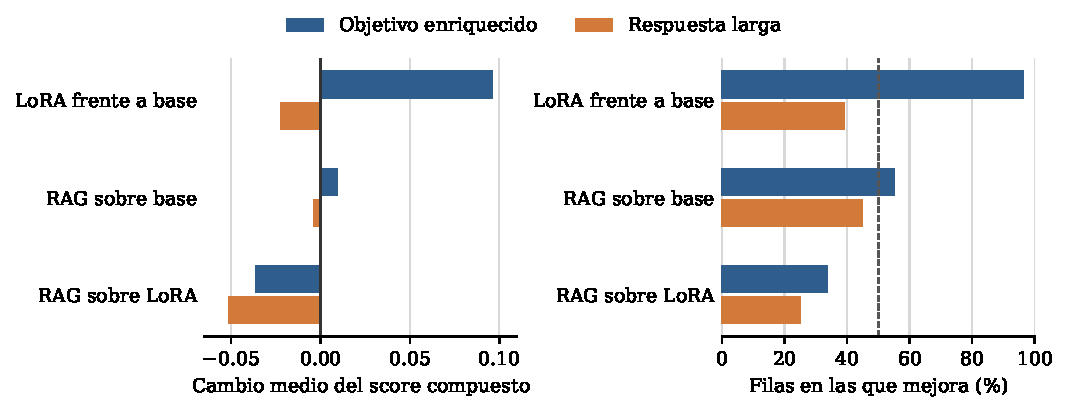
\includegraphics[width=0.88\textwidth]{figures/paired_effects.pdf}
\caption{Efectos pareados sobre el score compuesto por imagen. Un cambio positivo indica mejora respecto de la condición sin el componente evaluado; la línea punteada del panel derecho marca 50\% de filas.}
\label{fig:paired}
\end{figure*}

Los campos \texttt{explanation} ayudan a formular hipótesis sobre estos resultados. En el target enriquecido, el modelo base suele producir negativas genéricas, diferenciales abiertos y respuestas de unas 100 palabras; LoRA adopta una estructura clínica más estable y cercana a las 32,6 palabras de las referencias contrastivas. La mejora refleja, sobre todo, alineación de longitud, vocabulario y estructura con una supervisión homogénea. No demuestra por sí sola mejor razonamiento visual: la evidencia descrita por el analista continúa siendo a menudo genérica y existen respuestas convincentes con entidades diagnósticas incorrectas.

En respuesta larga ocurre el patrón inverso. Las referencias contrastivas promedian 87,4 palabras y mezclan etiquetas breves con narrativas extensas. El modelo base conserva más antecedentes y advertencias, mientras LoRA pierde cobertura o genera listas repetitivas. Los racionales también muestran que RAG puede arrastrar diagnósticos y tratamientos de casos vecinos. En \texttt{ENC00916}, por ejemplo, LoRA se aproxima a tiña versicolor, pero LoRA+RAG deriva hacia psoriasis y rosácea; el adapter RAG-aware vuelve a una hipótesis fúngica. En \texttt{ENC00965}, en cambio, una redacción clínicamente plausible oculta un diagnóstico incompatible con la referencia. Por ello tratamos estas explicaciones como evidencia post-hoc sobre patrones de salida, nunca como validación clínica ni como trazas causales.

\subsection{Eficiencia y auditoría clínica}

Los entrenamientos pareados de LoRA tardaron 77,3 minutos para el target enriquecido y 78,9 para respuesta larga en una NVIDIA L4; los picos de VRAM fueron 6,73 y 5,11 GB. El adapter RAG-aware tardó 108,3 minutos y alcanzó 5,67 GB. Cada adapter ocupa aproximadamente 160 MB y ajusta 37,2 millones de parámetros (0,98\% del modelo).

La auditoría exploratoria de 20 casos enriquecidos etiquetó 3 respuestas como correctas, 9 como parciales y 8 como incorrectas; además señaló 9 recomendaciones no sustentadas y 2 potencialmente inseguras. La muestra fue seleccionada por modos de error y las etiquetas fueron asistidas por IA, por lo que estos números solo ilustran riesgos. Los ejemplos muestran diagnósticos plausibles pero equivocados, omisión de diferenciales relevantes y tratamientos no presentes en la referencia.

\section{Discusión}

La respuesta a RQ1 es condicionada: bajo el mismo cómputo, LoRA aprende mucho mejor el objetivo enriquecido que la respuesta más larga. La síntesis reduce longitud, redundancia y contradicciones de estilo, y convierte múltiples opiniones en una señal supervisada más estable. Sin embargo, las métricas se calculan contra referencias distintas; no demuestran que la síntesis sea médicamente más verdadera.

Para RQ2, la adaptación eficiente sí supera al modelo base en el target enriquecido, pero no constituye una mejora universal. En respuesta larga, el modelo base conserva mayor similitud semántica. La calidad del target parece dominar la utilidad del fine-tuning.

Para RQ3, RAG ofrece mejoras pequeñas al modelo base enriquecido, pero empeora los adapters cuando se agrega únicamente en inferencia. Entrenar con el prompt RAG reduce ese desajuste y recupera BERTScore, aunque todavía no supera a LoRA simple. El análisis de \texttt{explanation} refuerza una interpretación concreta: recuperar por similitud de pregunta no garantiza similitud clínica, y los casos vecinos pueden aportar diagnósticos o tratamientos de otro paciente. La comparación aislada de recuperadores (Tabla~\ref{tab:retrieval}) muestra que la fusión texto+imagen no supera a su mejor componente individual con late fusion simple; un paso futuro es explorar representaciones multimodales conjuntas y filtrar evidencia por entidad diagnóstica, localización y morfología.

\section{Conclusiones}

Comparamos inferencia zero-shot, QLoRA/LoRA y RAG para VQA dermatológico en español. El mejor resultado automático corresponde a Qwen2.5-VL-3B adaptado sobre respuestas enriquecidas sin RAG. La misma receta sobre respuestas originales largas no mejora al modelo base, y el contexto recuperado tiende a perjudicar a LoRA. Por lo tanto, diseñar un objetivo supervisado consistente es una decisión central, no un detalle de preprocesamiento. Los errores cualitativos impiden interpretar el sistema como asistente clínico listo para uso real.

\section*{Limitaciones}

El test contiene 100 encuentros; las 314 imágenes no son observaciones independientes. No ejecutamos múltiples semillas ni intervalos de confianza agrupados por encuentro, por lo que las diferencias pequeñas no implican significancia estadística. El target enriquecido es sintético y puede consolidar errores de las respuestas originales o del LLM. La auditoría clínica y la muestra de explicaciones son dirigidas y no fueron validadas por dermatólogos; además, el analista externo no recibió el ground truth. Solo evaluamos Qwen2.5-VL-3B por restricciones de cómputo; para RAG usamos exclusivamente \texttt{multilingual-e5-small} (la Tabla~\ref{tab:retrieval} compara recuperadores de forma aislada, pero no probamos SBERT ni visual dentro del ciclo RAG) y un único valor de $k$. La condición RAG-aware no se entrenó sobre respuesta larga. Finalmente, las métricas de similitud textual no miden seguridad, calibración ni validez diagnóstica.

\section*{Consideraciones éticas}

Las consultas dermatológicas contienen información sensible y provienen de un dataset público preexistente; este trabajo hereda sus decisiones de anonimización y licencia. No intentamos identificar pacientes. El modelo puede producir diagnósticos o recomendaciones convincentes pero incorrectos, con riesgo de retrasar atención o inducir automedicación. Los artefactos se presentan exclusivamente para investigación y no deben usarse para diagnóstico ni tratamiento sin supervisión clínica, evaluación prospectiva y controles de privacidad.

\section*{Reproducibilidad}

El repositorio versiona scripts, configuraciones, predicciones y métricas ligeras. Las imágenes, claves y adapters no se publican. Los datasets se reconstruyen con los scripts de \texttt{src/}; las corridas VLM usan semilla 42 y guardan configuración, historial, métricas y tiempos. El manuscrito se compila localmente con \texttt{latexmk -pdf main.tex} desde \texttt{paper/acl}.

\bibliography{references}

\end{document}
